% Generated with:
% $ java -jar plantuml.jar -tlatex:nopreamble state-diagram.pu
% generated by Plantuml 1.2024.8       
\definecolor{plantucolor0000}{RGB}{241,241,241}
\definecolor{plantucolor0001}{RGB}{24,24,24}
\definecolor{plantucolor0002}{RGB}{0,0,0}
\definecolor{plantucolor0003}{RGB}{34,34,34}
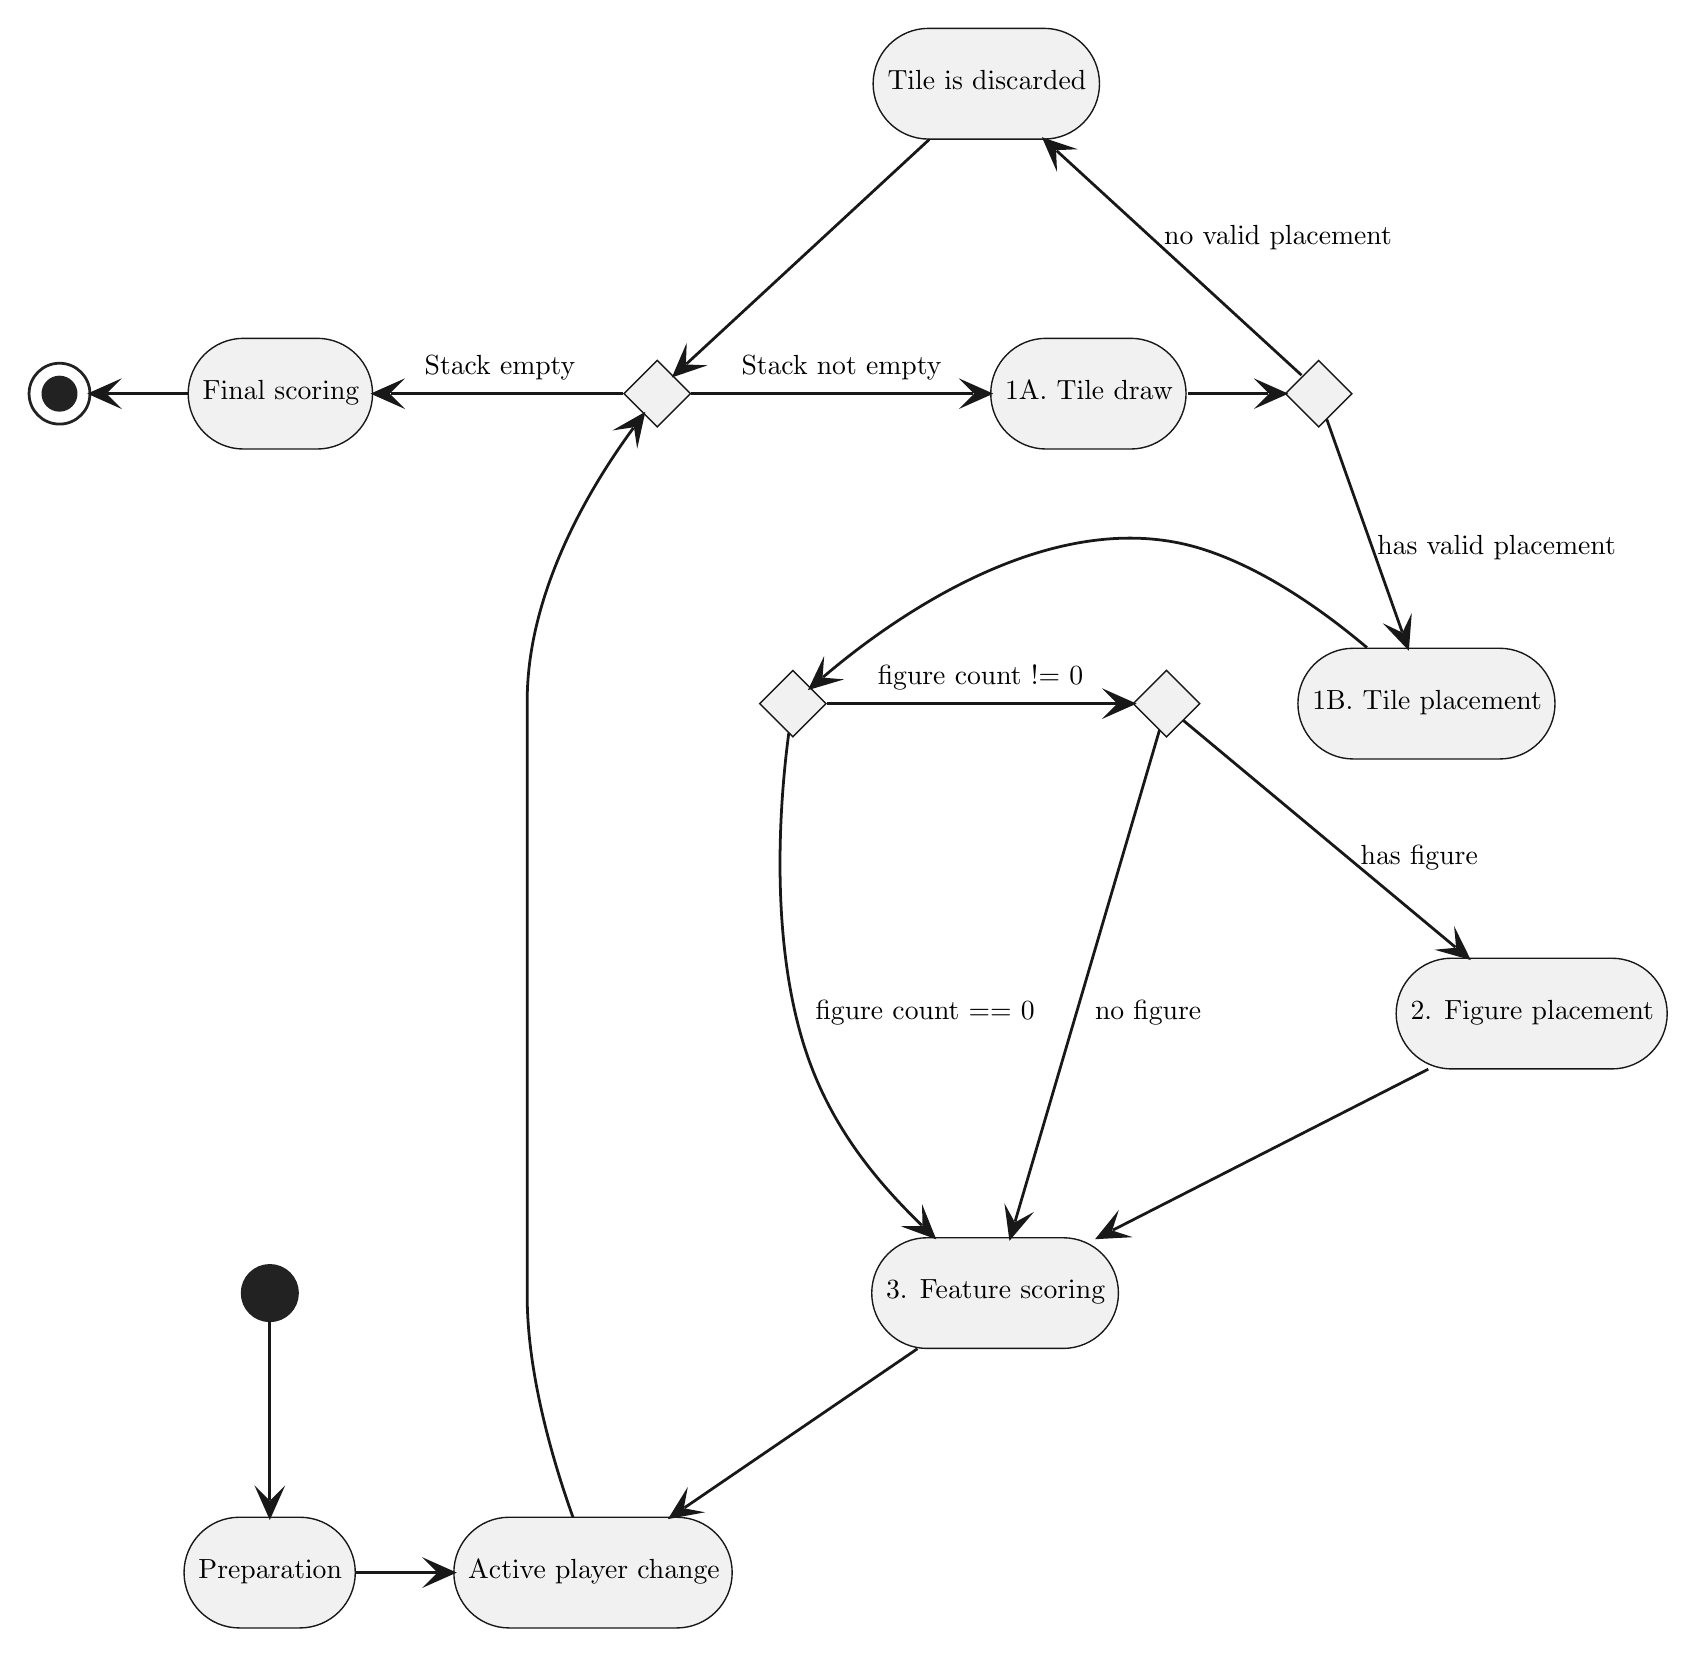
\begin{tikzpicture}[yscale=-1
,pstyle0/.style={color=plantucolor0001,fill=plantucolor0000,line width=0.5pt}
,pstyle1/.style={color=plantucolor0003,fill=plantucolor0003,line width=1.0pt}
,pstyle3/.style={color=plantucolor0001,line width=1.0pt}
,pstyle4/.style={color=plantucolor0001,fill=plantucolor0001,line width=1.0pt}
]
\draw[pstyle0] (159.5pt,565pt) arc (180:270:20pt) -- (179.5pt,545pt) -- (240.07pt,545pt) arc (270:360:20pt) -- (260.07pt,565pt) -- (260.07pt,565pt) arc (0:90:20pt) -- (240.07pt,585pt) -- (179.5pt,585pt) arc (90:180:20pt) -- (159.5pt,565pt) -- cycle;
\node at (164.5pt,560pt)[below right,color=black,inner sep=0]{Active player change};
\draw[pstyle0] (353.5pt,139pt) arc (180:270:20pt) -- (373.5pt,119pt) -- (404.08pt,119pt) arc (270:360:20pt) -- (424.08pt,139pt) -- (424.08pt,139pt) arc (0:90:20pt) -- (404.08pt,159pt) -- (373.5pt,159pt) arc (90:180:20pt) -- (353.5pt,139pt) -- cycle;
\node at (358.5pt,134pt)[below right,color=black,inner sep=0]{1A. Tile draw};
\draw[pstyle0] (233pt,127pt) -- (245pt,139pt) -- (233pt,151pt) -- (221pt,139pt) -- (233pt,127pt) -- cycle;
\draw[pstyle0] (311pt,27pt) arc (180:270:20pt) -- (331pt,7pt) -- (372.8pt,7pt) arc (270:360:20pt) -- (392.8pt,27pt) -- (392.8pt,27pt) arc (0:90:20pt) -- (372.8pt,47pt) -- (331pt,47pt) arc (90:180:20pt) -- (311pt,27pt) -- cycle;
\node at (316pt,22pt)[below right,color=black,inner sep=0]{Tile is discarded};
\draw[pstyle0] (472pt,127pt) -- (484pt,139pt) -- (472pt,151pt) -- (460pt,139pt) -- (472pt,127pt) -- cycle;
\draw[pstyle0] (464.5pt,251pt) arc (180:270:20pt) -- (484.5pt,231pt) -- (537.4pt,231pt) arc (270:360:20pt) -- (557.4pt,251pt) -- (557.4pt,251pt) arc (0:90:20pt) -- (537.4pt,271pt) -- (484.5pt,271pt) arc (90:180:20pt) -- (464.5pt,251pt) -- cycle;
\node at (469.5pt,246pt)[below right,color=black,inner sep=0]{1B. Tile placement};
\draw[pstyle0] (282pt,239pt) -- (294pt,251pt) -- (282pt,263pt) -- (270pt,251pt) -- (282pt,239pt) -- cycle;
\draw[pstyle0] (417pt,239pt) -- (429pt,251pt) -- (417pt,263pt) -- (405pt,251pt) -- (417pt,239pt) -- cycle;
\draw[pstyle0] (500pt,363pt) arc (180:270:20pt) -- (520pt,343pt) -- (577.94pt,343pt) arc (270:360:20pt) -- (597.94pt,363pt) -- (597.94pt,363pt) arc (0:90:20pt) -- (577.94pt,383pt) -- (520pt,383pt) arc (90:180:20pt) -- (500pt,363pt) -- cycle;
\node at (505pt,358pt)[below right,color=black,inner sep=0]{2. Figure placement};
\draw[pstyle0] (310.5pt,464pt) arc (180:270:20pt) -- (330.5pt,444pt) -- (379.64pt,444pt) arc (270:360:20pt) -- (399.64pt,464pt) -- (399.64pt,464pt) arc (0:90:20pt) -- (379.64pt,484pt) -- (330.5pt,484pt) arc (90:180:20pt) -- (310.5pt,464pt) -- cycle;
\node at (315.5pt,459pt)[below right,color=black,inner sep=0]{3. Feature scoring};
\draw[pstyle0] (63.5pt,139pt) arc (180:270:20pt) -- (83.5pt,119pt) -- (110.12pt,119pt) arc (270:360:20pt) -- (130.12pt,139pt) -- (130.12pt,139pt) arc (0:90:20pt) -- (110.12pt,159pt) -- (83.5pt,159pt) arc (90:180:20pt) -- (63.5pt,139pt) -- cycle;
\node at (68.5pt,134pt)[below right,color=black,inner sep=0]{Final scoring};
\draw[pstyle1] (93pt,464pt) ellipse (10pt and 10pt);
\draw[pstyle0] (62pt,565pt) arc (180:270:20pt) -- (82pt,545pt) -- (103.88pt,545pt) arc (270:360:20pt) -- (123.88pt,565pt) -- (123.88pt,565pt) arc (0:90:20pt) -- (103.88pt,585pt) -- (82pt,585pt) arc (90:180:20pt) -- (62pt,565pt) -- cycle;
\node at (67pt,560pt)[below right,color=black,inner sep=0]{Preparation};
\draw[color=plantucolor0003,line width=1.0pt] (17pt,139pt) ellipse (11pt and 11pt);
\draw[pstyle1] (17pt,139pt) ellipse (6pt and 6pt);
\draw[pstyle3] (93pt,474.14pt) ..controls (93pt,490.12pt) and (93pt,517.49pt) .. (93pt,538.77pt);
\draw[pstyle4] (93pt,544.77pt) -- (97pt,535.77pt) -- (93pt,539.77pt) -- (89pt,535.77pt) -- (93pt,544.77pt) -- cycle;
\draw[pstyle3] (124.08pt,565pt) ..controls (135.83pt,565pt) and (141.57pt,565pt) .. (153.32pt,565pt);
\draw[pstyle4] (159.32pt,565pt) -- (150.32pt,561pt) -- (154.32pt,565pt) -- (150.32pt,569pt) -- (159.32pt,565pt) -- cycle;
\draw[pstyle3] (202.54pt,544.98pt) ..controls (195.49pt,525.29pt) and (186pt,493.47pt) .. (186pt,465pt) ..controls (186pt,250pt) and (186pt,250pt) .. (186pt,250pt) ..controls (186pt,207.63pt) and (212.2854pt,167.7663pt) .. (224.4054pt,151.3563pt);
\draw[pstyle4] (227.97pt,146.53pt) -- (219.4055pt,151.3931pt) -- (224.9995pt,150.552pt) -- (225.8406pt,156.1459pt) -- (227.97pt,146.53pt) -- cycle;
\draw[pstyle3] (245.24pt,139pt) ..controls (268.23pt,139pt) and (312.64pt,139pt) .. (347.21pt,139pt);
\draw[pstyle4] (353.21pt,139pt) -- (344.21pt,135pt) -- (348.21pt,139pt) -- (344.21pt,143pt) -- (353.21pt,139pt) -- cycle;
\node at (263.25pt,125pt)[below right,color=black,inner sep=0]{Stack not empty};
\draw[pstyle3] (136.62pt,139pt) ..controls (165.88pt,139pt) and (200.67pt,139pt) .. (220.78pt,139pt);
\draw[pstyle4] (130.62pt,139pt) -- (139.62pt,143pt) -- (135.62pt,139pt) -- (139.62pt,135pt) -- (130.62pt,139pt) -- cycle;
\node at (148.75pt,125pt)[below right,color=black,inner sep=0]{Stack empty};
\draw[pstyle3] (424.66pt,139pt) ..controls (436.37pt,139pt) and (442.09pt,139pt) .. (453.8pt,139pt);
\draw[pstyle4] (459.8pt,139pt) -- (450.8pt,135pt) -- (454.8pt,139pt) -- (450.8pt,143pt) -- (459.8pt,139pt) -- cycle;
\draw[pstyle3] (377.3231pt,51.2142pt) ..controls (405.2631pt,76.8242pt) and (448.8pt,116.73pt) .. (465.8pt,132.32pt);
\draw[pstyle4] (372.9pt,47.16pt) -- (376.8318pt,56.19pt) -- (376.5859pt,50.5385pt) -- (382.2374pt,50.2926pt) -- (372.9pt,47.16pt) -- cycle;
\node at (416pt,78pt)[below right,color=black,inner sep=0]{no valid placement};
\draw[pstyle3] (331.27pt,47.16pt) ..controls (303.57pt,72.77pt) and (260.4153pt,112.6565pt) .. (243.5553pt,128.2465pt);
\draw[pstyle4] (239.15pt,132.32pt) -- (248.4736pt,129.1467pt) -- (242.8211pt,128.9254pt) -- (243.0423pt,123.2729pt) -- (239.15pt,132.32pt) -- cycle;
\draw[pstyle3] (474.93pt,148.27pt) ..controls (481.1pt,165.66pt) and (493.5342pt,200.7452pt) .. (502.1642pt,225.0752pt);
\draw[pstyle4] (504.17pt,230.73pt) -- (504.9312pt,220.9106pt) -- (502.4985pt,226.0177pt) -- (497.3914pt,223.585pt) -- (504.17pt,230.73pt) -- cycle;
\node at (493pt,190pt)[below right,color=black,inner sep=0]{has valid placement};
\draw[pstyle3] (489.44pt,230.75pt) ..controls (474.04pt,217.75pt) and (452.13pt,202.02pt) .. (429.5pt,195pt) ..controls (373.78pt,177.7pt) and (313.2289pt,224.0591pt) .. (292.9289pt,241.4291pt);
\draw[pstyle4] (288.37pt,245.33pt) -- (297.8089pt,242.518pt) -- (292.1691pt,242.0793pt) -- (292.6077pt,236.4395pt) -- (288.37pt,245.33pt) -- cycle;
\draw[pstyle3] (280.53pt,261.64pt) ..controls (277.54pt,283.91pt) and (272.38pt,340.35pt) .. (289pt,383pt) ..controls (298.28pt,406.82pt) and (313.2619pt,424.6538pt) .. (328.6119pt,439.5338pt);
\draw[pstyle4] (332.92pt,443.71pt) -- (329.242pt,434.5737pt) -- (329.3299pt,440.2299pt) -- (323.6738pt,440.3178pt) -- (332.92pt,443.71pt) -- cycle;
\node at (290pt,358pt)[below right,color=black,inner sep=0]{figure count == 0};
\draw[pstyle3] (294.46pt,251pt) ..controls (320.31pt,251pt) and (373.48pt,251pt) .. (398.96pt,251pt);
\draw[pstyle4] (404.96pt,251pt) -- (395.96pt,247pt) -- (399.96pt,251pt) -- (395.96pt,255pt) -- (404.96pt,251pt) -- cycle;
\node at (312.5pt,237pt)[below right,color=black,inner sep=0]{figure count != 0};
\draw[pstyle3] (414.49pt,260.53pt) ..controls (405.34pt,291.68pt) and (375.2818pt,393.9735pt) .. (362.2918pt,438.1735pt);
\draw[pstyle4] (360.6pt,443.93pt) -- (366.9754pt,436.423pt) -- (362.0098pt,439.1329pt) -- (359.3pt,434.1673pt) -- (360.6pt,443.93pt) -- cycle;
\node at (391pt,358pt)[below right,color=black,inner sep=0]{no figure};
\draw[pstyle3] (423.01pt,257.01pt) ..controls (440.97pt,271.97pt) and (490.2504pt,313.0492pt) .. (521.4304pt,339.0292pt);
\draw[pstyle4] (526.04pt,342.87pt) -- (521.6862pt,334.0357pt) -- (522.1987pt,339.6693pt) -- (516.5651pt,340.1818pt) -- (526.04pt,342.87pt) -- cycle;
\node at (487pt,302pt)[below right,color=black,inner sep=0]{has figure};
\draw[pstyle3] (511.59pt,383.09pt) ..controls (477.24pt,400.62pt) and (431.9546pt,423.7332pt) .. (397.6346pt,441.2432pt);
\draw[pstyle4] (392.29pt,443.97pt) -- (402.1247pt,443.4429pt) -- (396.7438pt,441.6977pt) -- (398.489pt,436.3167pt) -- (392.29pt,443.97pt) -- cycle;
\draw[pstyle3] (327.04pt,484.09pt) ..controls (301.37pt,501.62pt) and (268.4754pt,524.0772pt) .. (242.8254pt,541.5872pt);
\draw[pstyle4] (237.87pt,544.97pt) -- (247.5584pt,543.1994pt) -- (241.9995pt,542.151pt) -- (243.0479pt,536.5921pt) -- (237.87pt,544.97pt) -- cycle;
\draw[pstyle3] (34.25pt,139pt) ..controls (45.98pt,139pt) and (51.7pt,139pt) .. (63.43pt,139pt);
\draw[pstyle4] (28.25pt,139pt) -- (37.25pt,143pt) -- (33.25pt,139pt) -- (37.25pt,135pt) -- (28.25pt,139pt) -- cycle;
\end{tikzpicture}
